% Options for packages loaded elsewhere
\PassOptionsToPackage{unicode}{hyperref}
\PassOptionsToPackage{hyphens}{url}
%
\documentclass[
]{book}
\usepackage{amsmath,amssymb}
\usepackage{lmodern}
\usepackage{iftex}
\ifPDFTeX
  \usepackage[T1]{fontenc}
  \usepackage[utf8]{inputenc}
  \usepackage{textcomp} % provide euro and other symbols
\else % if luatex or xetex
  \usepackage{unicode-math}
  \defaultfontfeatures{Scale=MatchLowercase}
  \defaultfontfeatures[\rmfamily]{Ligatures=TeX,Scale=1}
\fi
% Use upquote if available, for straight quotes in verbatim environments
\IfFileExists{upquote.sty}{\usepackage{upquote}}{}
\IfFileExists{microtype.sty}{% use microtype if available
  \usepackage[]{microtype}
  \UseMicrotypeSet[protrusion]{basicmath} % disable protrusion for tt fonts
}{}
\makeatletter
\@ifundefined{KOMAClassName}{% if non-KOMA class
  \IfFileExists{parskip.sty}{%
    \usepackage{parskip}
  }{% else
    \setlength{\parindent}{0pt}
    \setlength{\parskip}{6pt plus 2pt minus 1pt}}
}{% if KOMA class
  \KOMAoptions{parskip=half}}
\makeatother
\usepackage{xcolor}
\IfFileExists{xurl.sty}{\usepackage{xurl}}{} % add URL line breaks if available
\IfFileExists{bookmark.sty}{\usepackage{bookmark}}{\usepackage{hyperref}}
\hypersetup{
  pdftitle={Lab Manual for the No Name Lab},
  pdfauthor={The Lab},
  hidelinks,
  pdfcreator={LaTeX via pandoc}}
\urlstyle{same} % disable monospaced font for URLs
\usepackage{longtable,booktabs,array}
\usepackage{calc} % for calculating minipage widths
% Correct order of tables after \paragraph or \subparagraph
\usepackage{etoolbox}
\makeatletter
\patchcmd\longtable{\par}{\if@noskipsec\mbox{}\fi\par}{}{}
\makeatother
% Allow footnotes in longtable head/foot
\IfFileExists{footnotehyper.sty}{\usepackage{footnotehyper}}{\usepackage{footnote}}
\makesavenoteenv{longtable}
\usepackage{graphicx}
\makeatletter
\def\maxwidth{\ifdim\Gin@nat@width>\linewidth\linewidth\else\Gin@nat@width\fi}
\def\maxheight{\ifdim\Gin@nat@height>\textheight\textheight\else\Gin@nat@height\fi}
\makeatother
% Scale images if necessary, so that they will not overflow the page
% margins by default, and it is still possible to overwrite the defaults
% using explicit options in \includegraphics[width, height, ...]{}
\setkeys{Gin}{width=\maxwidth,height=\maxheight,keepaspectratio}
% Set default figure placement to htbp
\makeatletter
\def\fps@figure{htbp}
\makeatother
\setlength{\emergencystretch}{3em} % prevent overfull lines
\providecommand{\tightlist}{%
  \setlength{\itemsep}{0pt}\setlength{\parskip}{0pt}}
\setcounter{secnumdepth}{5}
\usepackage{booktabs}
\ifLuaTeX
  \usepackage{selnolig}  % disable illegal ligatures
\fi
\usepackage[]{natbib}
\bibliographystyle{apalike}

\title{Lab Manual for the No Name Lab}
\author{The Lab}
\date{Updated on 2022-06-20}

\begin{document}
\maketitle

{
\setcounter{tocdepth}{1}
\tableofcontents
}
\hypertarget{welcome}{%
\chapter*{Welcome!}\label{welcome}}
\addcontentsline{toc}{chapter}{Welcome!}

Welcome to the No-Name Lab at the University of Wisconsin, Parkside! If you are reading our lab manual because you recently joined the lab, welcome! If you are a current member of the lab, frequently refer to our lab manual to refresh our guidelines, policies, platforms, among others. We also look forward to learn and research together. We also welcome you to read this manual if you are looking for tips and tricks for your own manual.

It's also a work in progress; therefore, updates are implemented as we move forward. If you have ideas about things to add, or what to clarify, feel free to talk to the PI (Dr.~Jordan Snyder).

No Name lab members are expected to read this manual and sign a form within your first 7 days in the lab indicating you have done so. Signing this form confirms that the lab member will perform their duties and meet the expectations according to this manual.

Before the actual lab manual, we have some people to thank. These include folks who have made their lab manual accessible and members of the lab who have provided feedback based upon the lab manual. Some of the sections are taken directly from these sources, and all of them have provided inspiration on aspects to include in this manual.

Specifically, we thank the following for making their lab manuals accessible:

\begin{itemize}
\item
  \href{https://github.com/alylab/labmanual/blob/master/aly-lab-manual.pdf}{Dr.~Aly's Aly Lab Manual}, who was also kind enough to write up an article about the lab manual \citep{aly2018key}
\item
  \href{https://osf.io/pwnsm/}{Dr.~Schleider's Lab Manual for the Lab for Scalable Mental Health}
\item
  \href{https://www.thecollablab.org/}{Dr.~Treichler's Collab Lab Manual}
\item
  \href{http://www.saraemilyburke.com/IntergroupBiasLabManual.pdf}{Dr.~Burke's Inergroup Bias Lab Manual}
\item
  \href{https://bookdown.org/friveram/labmanualriplrt/}{Dr.~Rivera-Mariani's RIPLRT Lab Manual}
\end{itemize}

\hypertarget{about-this-lab-manual}{%
\section{About this Lab Manual}\label{about-this-lab-manual}}

We use a lab manual for a few reasons. First, it makes certain things explicit, including things like expectations, so that we don't have to guess. Second, it removes the informal passing on of critical information; with this information and the appropriate information in the \href{}{LAB WIKI - LINK TBD}, you should have everything to get caught up to reasonable speed. If you do find something that you think is necessary, but not in here, talk with Jordan or the lab manager about getting this added.

Jordan will likely revise this lab manual on an semester basis, and as issues come up.

\textbf{Welcome to the Lab!}

\emph{Note: the date listed above corresponds to the date the manual was updated. The date this manual was initially created was on {[}INSERT DATE HERE{]}.}

\begin{center}\rule{0.5\linewidth}{0.5pt}\end{center}

\textbf{Note}: The repository for this lab manual can be found here: \url{https://github.com/jordandsnyder/labmanual}. Also, this manual was developed, and continuously updated (as needed), through the R \citep{R-base} computer language, and employs the Bookdown \citep{R-bookdown}, knitr \citep{R-knitr}, and R-markdown \citep{R-rmarkdown} packages.

\hypertarget{about-the-lab}{%
\chapter{About the Lab}\label{about-the-lab}}

\hypertarget{mission}{%
\section{Mission}\label{mission}}

The Lab seeks to serve, empower, and equip individuals and communities to answer their questions, meet their objectives, and transform their lives and communities using community-based mixed methods psychological research. We are particularly interested in working with communities traditionally underserved by clinical psychology, and in particular folks and communities affected by conflict, broadly construed. Wherever we work, we strive to do our work with integrity, humility, and in the context of authentic relationships.

\hypertarget{vision}{%
\section{Vision}\label{vision}}

We seek to partner with communities and work towards community health and wellness in the world, one community at a time.

\hypertarget{core-values}{%
\section{Core Values}\label{core-values}}

These are values that guide and direct our work on a daily basis. By working in the lab, we all agree to work towards these values.

\begin{itemize}
\item
  Humility: We seek to be open to learning new things through trying out and making mistakes. We will own up to mistakes, and learn from them.
\item
  Curiosity: We approach situations as opportunities to learn something new.
\item
  Integrity: We say what we mean, and mean what we say. We do what we say we will do, and admit when we have made mistakes.
\item
  Relationships: We work towards forming authentic relationships with each other and community partners.
\item
  Persistence: We try, try, and try again.
\item
  Service: We look to the interests of others, including fellow labmates, community partners, and research participants.
\item
  Diversity: We all have different backgrounds and experiences. Through this diversity, we can all learn and get a better perspective.
\end{itemize}

\hypertarget{the-communities-with-whom-we-partner}{%
\section{The Communities with whom we partner}\label{the-communities-with-whom-we-partner}}

While open to working with a diverse range of communities, we have traditionally worked to improve wellness in conflict-affected populations. Specifically, we have partnered with the following organizations:

\begin{itemize}
\item
  \href{https://www.carsaministry.org/}{Christian Action for Reconciliation and Social Assistance (CARSA)} - a nonprofit organization in Rwanda working to heal communities in the aftermath of the 1994 Rwandan genocide.
\item
  \href{warmalska.org}{Working Alongside Refugees in Mental Health (WARM)} - a network of mental health providers and allied organizations working to train mental health providers to work with forced migrants, like refugees and asylum-seekers.
\end{itemize}

\hypertarget{our-collaborators}{%
\section{Our Collaborators}\label{our-collaborators}}

Another crucial part of work are those with whom we collaborate. We believe that science is better (and more enjoyable) when done with partners. Below are a couple of our collaborators:

\begin{itemize}
\item
  \href{https://www.uaa.alaska.edu/academics/college-of-arts-and-sciences/departments/psychology/faculty/buckingham.cshtml}{Sara Buckingham, Ph.D.}, and the \href{https://crossroadsresearch.wixsite.com/collective}{Crossroads Research Collective}
\item
  \href{https://profiles.howard.edu/profile/466/ezer-kang}{Ezer Kang, Ph.D.}, and the \href{https://ezerkang-howard-faculty.com/}{Global Community Health Lab}
\end{itemize}

\hypertarget{our-history}{%
\section{Our History}\label{our-history}}

Jordan established the lab in 2022 at UW Parkside. Kaylie Garcia and Rachael Hall were inaugural lab members beginning in Spring 2022 and Undergraduate Research Assistants through the \protect\hyperlink{URAP}{Undergraduate Research Aassistantship Program (URAP)} in Summer 2022.

\hypertarget{space-and-info}{%
\section{Space and Info}\label{space-and-info}}

The lab is located at the University of Wisconsin Parkside, and a physical location is MOLN315E. Information about accessing the lab is available from Jordan.

Lab Website: TBD
Lab Wiki: TBD
Lab Manual: TBD

PI contact: TB

\hypertarget{joining-the-lab}{%
\section{Joining the Lab}\label{joining-the-lab}}

To join the lab, there is a multi-step process.

\begin{enumerate}
\def\labelenumi{\arabic{enumi}.}
\tightlist
\item
  Send Jordan a lab application. A lab application consists of sending Jordan an email (\href{mailto:snyderj@uwp.edu}{\nolinkurl{snyderj@uwp.edu}}) with the following: (1) what year you will be in the semester/year you want to be an RA, (2) your expected month and year of graduation, (3) whether or not you have completed Statistics and Research Methods, (4) your GPA, (5) why you want to be an RA, and which type of RA you are interested in being (see below for more information, but options are for credit, volunteer, or URAP), (6) what area of psychology is most interesting to you and why, (7) what are your strengths and weaknesses, (8) what are your plans for the future, and (9) anything else you think is relevant. I will respond to your email and let you know if we should have an interview. Please note, there are several ways to join the lab:
\end{enumerate}

\begin{itemize}
\item
  Join the lab as a volunteer. If you join the lab as a volunteer, you will not get compensated or get academic credit for participating in lab. I ask students who volunteer in lab not to do more than 5 hours of lab work per week (inclusive of all meetings).
\item
  Join the lab for credit. If you join the lab for credit (and Jordan approves this), you will work on a form with Jordan to submit to the registrar. The form will contain a list of obligations/responsibilities for you to complete for a grade. You will get credit for \href{https://www.uwp.edu/learn/academiccatalog/2019-2021/psyc.cfm\#courses\#courses}{PSYC499}. You can get up to 6 credits of PSYC499, with 3 credits counting for upper level electives in the psychology major, and 3 credits counting for upper level electives. If you wish to use 6 credits, I ask that you commit to a full year in the lab (September - May) and use 3 credits per semester. I ask students to expect to work a maximum of 3 hours per week per credit hour (e.g., for 3 credits, you could work up to 9 hours in lab responsibilities per week). However, I don't want you working more than that outside special occasions (e.g., traveling to a conference, etc.).
\item
  Join the lab as through \protect\hyperlink{URAP}{the Undergraduate Research Assistantship Program (URAP)}. Typically, I encourage students to be in the lab before joining through the URAP program, as these applications are best done once you have been in the lab.
\end{itemize}

\begin{enumerate}
\def\labelenumi{\arabic{enumi}.}
\setcounter{enumi}{1}
\item
  Jordan will review these applications on a weekly basis and reach out if he has capacity/availability for a student to schedule an interview. Based upon the application and the interview, he may extend an invitation to join the lab.
\item
  If you join the lab, you will be expected to do the following:
\end{enumerate}

\begin{itemize}
\tightlist
\item
  Do the \href{}{Onboarding Section - LINK TBD} of this lab manual.
\item
  Fufill the obligations listed in the expectations role for which you are joining the lab.
\end{itemize}

\begin{enumerate}
\def\labelenumi{\arabic{enumi}.}
\setcounter{enumi}{3}
\tightlist
\item
  Jordan will do the following:
\end{enumerate}

\begin{itemize}
\tightlist
\item
  Add you to the lab sharepoint.
\item
  Review your individual mentoring plan with you.
\end{itemize}

\hypertarget{expectations-and-responsiblities}{%
\chapter{Expectations and Responsiblities}\label{expectations-and-responsiblities}}

\hypertarget{everyone}{%
\section{Expectations of Everyone}\label{everyone}}

\hypertarget{big-picture}{%
\subsection{Big Picture}\label{big-picture}}

\begin{itemize}
\item
  Do work that impacts folks and communities, and increases their wellness.
\item
  Do work that makes you proud; make sure the work you do is the highest-quality work you can do. Don't rush. Double-check things. Don't make careless mistakes.
\item
  Remember that you are human; you will make mistakes, and this is okay. If you make a mistake, tell someone early and often. The earlier we can catch a mistake, the easier it is to correct. Jordan has made many mistakes (and will make more mistakes in the future), but please speak up!
\item
  Related to the University of Wisconsin, Parkside's policies on academic integrity (\href{https://www.uwp.edu/explore/offices/governance/policy28.cfm}{Policy 28},\href{https://www.uwp.edu/explore/offices/governance/policy35.cfm}{Policy 35}), maintain integrity in doing scholastic and scientific work. Do not plagiarize, make up data, or alter results. The consequences of doing these can significant. If you have questions about this, talk to someone, including Jordan.
\item
  Support your lab-mates. Help them if needed, even if it is a different project. We all do better when we support each other.
\item
  Respect your lab-mates. Respect their strengths, their developing skills, and their culture, religion, beliefs, and identity.
\item
  If you are struggling, talk with someone! Feel free to talk with Jordan. Your health and wellness is the 1st priority. We look out for each other and understand that life can be difficult. Please feel free to ask for help, or just to talk through things. If you find yourself struggling with anything in lab, please tell Jordan, he values you more than the project that you are on.
\item
  If there is tension or hostility within the lab, we need to address this. Disrespect and rudeness is not acceptable. If you don't feel comfortable addressing the issue with the responsible party, talk with Jordan (even if you feel okay talking with the responsible party, it is still good to tell Jordan).
\item
  If you have an issue with Jordan, please talk to him about it. If you are not comfortable talking with Jordan, I encourage you to follow up with the department chair (currently Dr.~Gregg). She can offer guidance and, if appropriate, intervene on your behalf.
\item
  Outside of lab, please enjoy your life. Jordan would love to hear about cool things you are doing, what you are watching or reading, good places to eat, and where you are traveling to. Jordan believes that life is more than just work, and will lead by example (and share this with you). Jordan doesn't expect students to share about their life unless they want to, however.
\end{itemize}

\hypertarget{small-picture-every-day}{%
\subsection{Small Picture (every day)}\label{small-picture-every-day}}

\begin{itemize}
\item
  If you are sick, please stay home. Reschedule meetings, and you can work remotely if up against a deadline.
\item
  Please keep the lab space clean and tidy. Please clean up after yourself. Please be respectful of the equipment in the lab space.
\item
  Show up to your meetings, your lab hours, interviews/running participants or stakeholders, and lab meetings. Do what you say you will do (i.e., do what you have committed to doing and be dependable).
\item
  Dress code is casual. There are a couple exceptions including working in communities/conducting interviews (in which case, talk with Jordan) and presenting information (professional attire, talk with Jordan about this).
\item
  Lock the lab once you leave it. Turn off any lights/air conditioners if you are leaving.
\item
  Please be responsive to communication. When lab is in session (September to December; February to May), I expect email responses in 24-48 hours during the work week (Monday-Friday).
\item
  Work when you want, but keep track of the time you work so as to not exceed what your role entails. If you find yourself working over the hours prescribed for your role, please talk with Jordan. I don't expect you to work on weekends or late into the night. If this is continually happening, please talk with me.
\end{itemize}

\hypertarget{expectations-of-jordan}{%
\section{Expectations of Jordan}\label{expectations-of-jordan}}

Jordan will do everything in the \protect\hyperlink{everyone}{everyone section} and the following:

\begin{itemize}
\item
  Provide supportive, thoughtful, and individually-tailored guidance that is appropriate for your training level.
\item
  Prioritize your growth as a scientist. Jordan will do his best to support, guide, and collaborate on your work without micromanaging it. It is on you to see ideas through to completion.
\item
  Provide feedback on scientific products (abstracts, papers, pre-registrations, etc.). I will try to do this within a week, unless I have other commitments. I will let you know if this is the case.
\item
  Be available via email and in-person (either in human form or via Zoom) to discuss research, lab-related, and professional development topics.
\item
  Maintain a vision for where the lab is going.
\item
  Welcome feedback from lab members to improve the lab.
\item
  Help you prepare for what comes next for you.
\item
  Provide students with written feedback on their performance on an annual basis. If there is any issue, Jordan will provide feedback as soon as possible and help to address challenges collaboratively.
\item
  Obtain funding to support lab members and research projects.
\item
  Create an inclusive, supportive, and scientifically rigorous work culture where people and ideas are valued.
\item
  Geek out on stats and technology stuff related to labwork.
\item
  Care about you as a person.
\end{itemize}

\hypertarget{expectations-of-lab-manager}{%
\section{Expectations of Lab Manager}\label{expectations-of-lab-manager}}

The lab manager will do everything mentioned in the \protect\hyperlink{everyone}{everyone section} as well as the following:

\begin{itemize}
\item
  Assist in maintaining aspects of day-to-day lab functions, and work on other lab projects based on
  the lab's needs.
\item
  Help Jordan in coordinating the overall progress of the lab and its projects, and help Jordan coordinate any other research assistants.
\item
  Help maintain the lab website, lab wiki, lab manual, lab schedule/calendar, and other administrative tasks of the lab.
\item
  Focus on collecting high-quality data from our participants, with every participant you interact with. The quality of our research relies on the quality of our data. In other words: \emph{Your job is incredibly important!}
\item
  Maintain IRB protocols for the lab that are connected to the projects you work on.
\item
  Assist with data collection, cleaning, and analysis.
\item
  Help new lab members adjust to the lab by answering whatever questions you can. Jordan can fill-in gaps when you aren't sure about a particular answer.
\item
  Delegate tasks to undergraduate research assistants.
\item
  Contribute to day-to-day lab functions, update the lab website, and contribute to other studies and lab activities based on your interest and availability, and the lab's needs.
\item
  Develop an individualized training plan with my help (and potentially other members of the lab or other mentors) that will help you reach your professional goals (like going to graduate school).
\item
  Work with our clinical, community, and research partners, especially when it comes to managing study procedures, maintaining strong relationships, and troubleshooting problems.
\item
  Maintain IRB protocols for the studies you work on.
\item
  Monitor our resources, including printing, audio taping devices, transcriptions, assessments, and other things we need.
\item
  Identify and work on your own research projects, which may be a part of or offshoots of the study you were hired to work on, but could also be new research projects. Keep in mind that starting new projects can be time consuming, so if you would like to do this, make sure you plan to stay in your role long enough to complete data collection and analysis.
\item
  Participate in other activities that will help with your professional development. I can help you identify these as needed.
\end{itemize}

\hypertarget{expectations-of-project-leads}{%
\section{Expectations of Project Leads}\label{expectations-of-project-leads}}

The Project leads will do everything mentioned in the \protect\hyperlink{everyone}{everyone section} as well as the following:

\begin{itemize}
\item
  Focus primarily on the study or studies you joined for.
\item
  Serve as the lead of the project you are assigned to, which means you train and supervise the URAs assigned to your project as needed. Serve as the communicator to Jordan about what is happening with the project.
\item
  Contribute to day-to-day lab functions, and contribute to other studies and lab activities based on your interest and availability, and the lab's needs.
\item
  Develop an individualized training plan with my help (and potentially other members of the lab or other mentors) that will help you reach your professional goals (like going to graduate school).
\item
  Focus on collecting high-quality data from every participant you interact with, and otherwise uphold high levels of scientific and professional rigor. The quality of our research depends on the quality of our data. Data collection is an incredibly important role!
\item
  Meet regularly with your primary supervisor(s). Attend lab meetings, journal clubs, and other meetings.
\item
  Identify roles on existing or upcoming research projects. Work with the other members of the team to establish your role and authorship status on those projects.
\item
  Participate in other activities that will help with your professional development. I can help you identify these as needed.
\item
  Present at one lab meeting each year.
\item
  Present in some form at once conference.
\end{itemize}

\hypertarget{expectations-of-undergraduate-research-assistants-uras-volunteer-urap-for-credit}{%
\section{Expectations of Undergraduate Research Assistants (URAs; volunteer, URAP, for credit)}\label{expectations-of-undergraduate-research-assistants-uras-volunteer-urap-for-credit}}

The Undergraduate Research Assistant will do everything mentioned in the \protect\hyperlink{everyone}{everyone section} as well as the following:

\begin{itemize}
\item
  Focus primarily on the study or studies you joined for.
\item
  Contribute to day-to-day lab functions, and contribute to other studies and lab activities based on your interest and availability, and the lab's needs.
\item
  Develop an individualized training plan with my help (and potentially other members of the lab or other mentors) that will help you reach your professional goals (like going to graduate school).
\item
  Focus on collecting high-quality data from every participant you interact with, and otherwise uphold high levels of scientific and professional rigor. The quality of our research depends on the quality of our data. Data collection is an incredibly important role!
\item
  Meet regularly with your primary supervisor(s). Attend lab meetings, journal clubs, and other meetings.
\item
  Identify roles on existing or upcoming research projects. Work with the other members of the team to establish your role and authorship status on those projects.
\item
  Participate in other activities that will help with your professional development. I can help you identify these as needed.
\item
  Present at one lab meeting each year.
\item
  Present in some form at once conference.
\end{itemize}

\hypertarget{volunteer}{%
\subsubsection{Volunteer}\label{volunteer}}

Volunteer URA have a few stipulations:

\begin{itemize}
\tightlist
\item
  If you are a volunteer in the lab, you will limit your participation up to 5 hours, inclusive of all lab activities. Please tell Jordan if you are working more than this.
\end{itemize}

\hypertarget{urap}{%
\subsubsection{URAP}\label{urap}}

URAP URAs have a few stipulations:

\begin{itemize}
\item
  Keep up a diary of what you work on/accomplish so that you can use this when you write up your required report.
\item
  Expected hours are about 5 hours per week if you are being paid during the fall/spring semesters. If you are working more than this, tell Jordan.
\end{itemize}

\hypertarget{for-credit}{%
\subsubsection{For Credit}\label{for-credit}}

For Credit URAs have a few stipulations:

\begin{itemize}
\item
  Work with Jordan to turn in the forms needed for the registrar.
\item
  Do all of the tasks required in the form for your grade.
\item
  Expected hours are about 9 hours per week if you are doing the 3 credit version. If you are working more than this, tell Jordan.
\end{itemize}

\hypertarget{expectations-of-the-lab-mascot-nelson}{%
\section{Expectations of the Lab Mascot, Nelson}\label{expectations-of-the-lab-mascot-nelson}}

Nelson's expectations are to be cute and distract Jordan from writing by causing mischief.

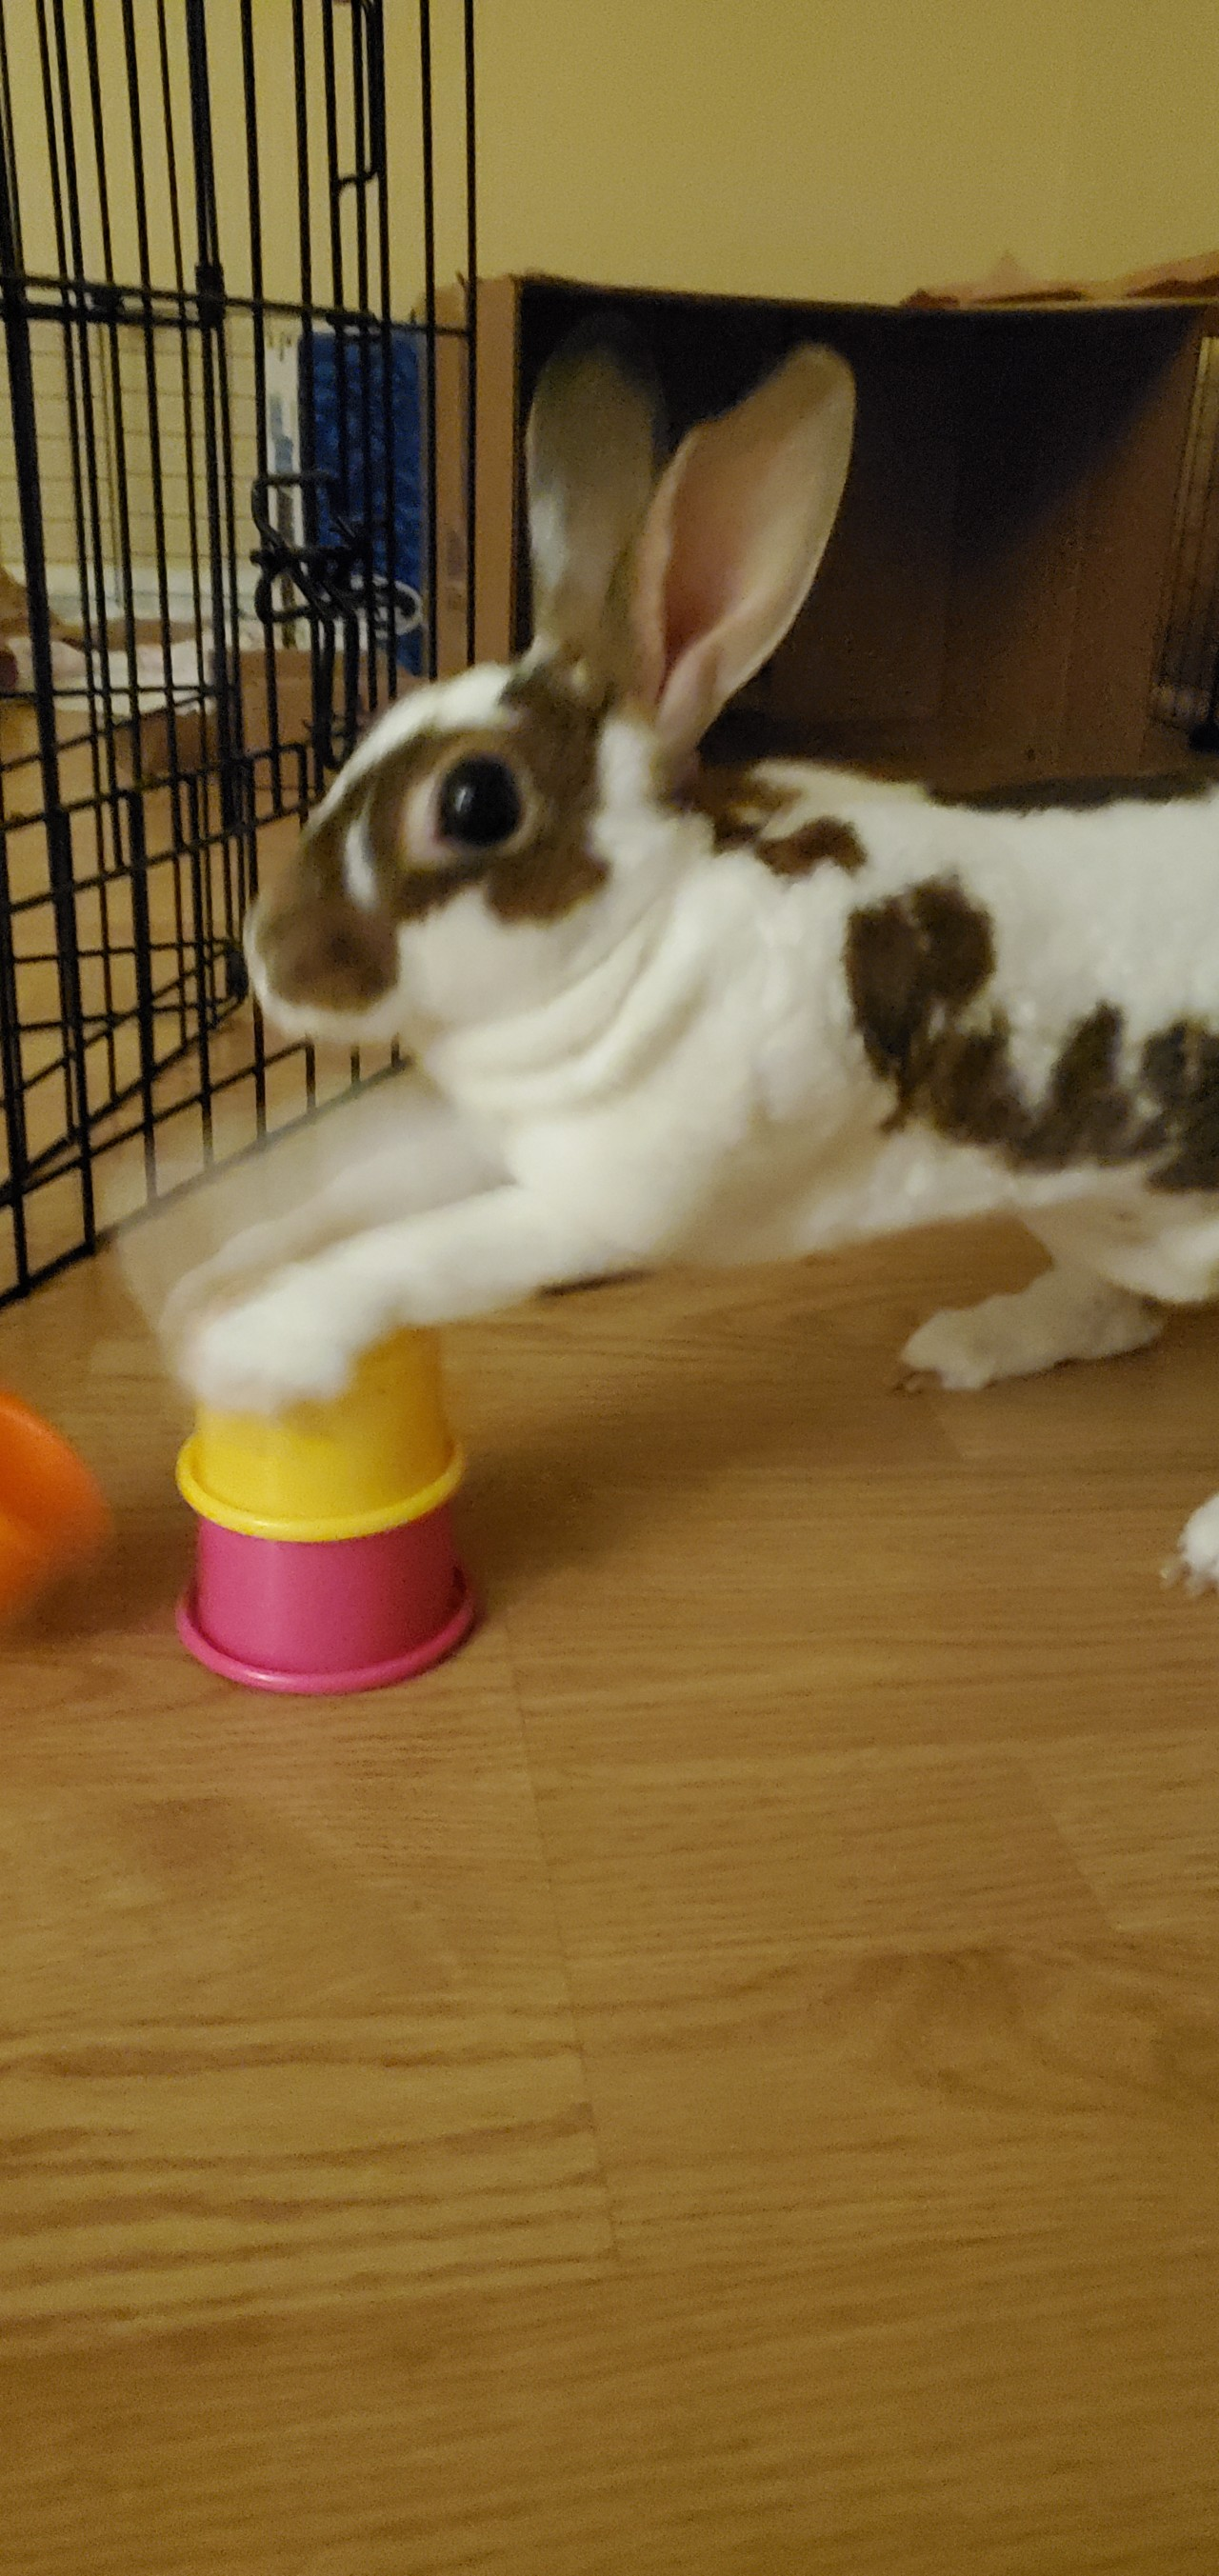
\includegraphics{images/nelsonplaying.jpg}

\hypertarget{code-of-conduct-and-policies}{%
\chapter{Code of Conduct and Policies}\label{code-of-conduct-and-policies}}

The lab is dedicated to providing a safe experience for everyone, regardless of race, ethnicity, gender identity and expression, age, sexual orientation, disability, mental health status, country of origin, or religious/spiritual beliefs. We do not tolerate harassment of lab members in any form. Harassment includes but is not limited to: offensive verbal comments, deliberate intimidation, stalking, following, harassing photography or recording, sustained disruption of talks, threats, coercive behavior, inappropriate physical contact, and unwelcome sexual attention. We expect all lab members to follow these guidelines at any lab-related event.

Lab members asked to stop harassing behavior are expected to comply immediately. Failure to comply could lead to consequences including dismissal from the lab, and/or legal action.

If you are being harassed, notice that someone else is being harassed, or have any other concerns, please contact Jordan immediately. If you have concerns about Jordan, please reach out to Dr.~Gregg or another trusted faculty member or administrator who can assist.

If you experience any form of sexual harassment, sex discrimination, or gender-based violence, you can file a report with the \href{https://www.uwp.edu/explore/offices/titleix/}{Title IX office at UWP}.

\textbf{IMPORTANT}: UWP Faculty members are considered ``responsible employees'' or ``mandated reporters,'' meaning that they are required to report violations of Title IX to the TItle IX Coordinator. Jordan is a responsible employee and must report any Title IX related incidents that are disclosed in writing, discussion, or a one-on-one. Before talking with Jordan about a Title IX incident, be sure to ask whether they are a responsible employee. Jordan is happy to talk with you and help you, but Jordan wants you to be certain you are aware of his status and are comfortable with him about reporting an incident you choose to disclose. Jordan will try to check with you if he gets the feeling you are about to disclose a Title IX violation. IF you wish to speak with someone for support or remedies without making an official report, you can talk to confidential services at the \href{https://www.uwp.edu/live/services/studenthealth/}{UWP Student Health and Counseling Center}. You can also talk to me without talking about specifics, and I can be glad to help connect you to care/support.

Please also know that Jordan is required to report any suspected child abuse/neglect as apart of his role as well. Please let him know if you have any questions or concerns.

\hypertarget{diversity-and-inclusion}{%
\section{Diversity and Inclusion}\label{diversity-and-inclusion}}

This lab is committed to an environment that is supportive, educational, and empowering for everyone. Thus, this lab is committed to diversity, inclusion, and equity for everyone regardless of group membership. This means the lab actively does the following (but this is a non-exhaustive list):

\begin{itemize}
\tightlist
\item
  Jordan seeks out ongoing education on how to work with students who belong to traditionally underrepresented groups in clinical psychology. He welcomes feedback from students, but he does not expect them to teach him how to teach them.
\item
  Jordan is committed to the ideas of cultural humility, and he will talk about this in lab quite a bit.
\item
  Jordan will seek out funding for students and scholars from traditionally underrepresented backgrounds in the lab's research.
\item
  We prioritize open, rigorous scientific methods, and communicating these results to those we partner with.
\item
  We seek to provide a culture of mutual support.
\item
  We commit to standing in solidarity with each other when we see discrimination and inappropriate behavior.
\end{itemize}

\hypertarget{problems-and-reporting}{%
\section{Problems and Reporting}\label{problems-and-reporting}}

If you have problems with another lab member, you can talk with them if it is something you feel comfortable with. If you do not feel comfortable with talking with the lab member, please talk with Jordan. If you have problems with Jordan, but do not wish to talk with Jordan about them (but please do if you feel comfortable sharing with me), feel free to talk to Dr.~Gregg or another trusted faculty member.

\hypertarget{academic-and-scientific-integrity}{%
\section{Academic and Scientific Integrity}\label{academic-and-scientific-integrity}}

The integrity of the research and work that we conduct is critical. This means that there is to be no fabrication, falsification, omission, characterization, plagiarism, `fudging', or any other unethical scientific/academic practices in the work that we do. If there is any academic dishonesty or scientific misconduct, it will be treated as a very serious matter, and there can be serious consequences for engaging in dishonesty or misconduct. If you are concerned about the academic or scientific practices happening in the lab, please talk with Jordan. If you are unfamiliar with policies, please talk with Jordan.

Please respect yourself, your peers, Jordan, and the communities and people we work with by refraining from any academic dishonesty and scientific misconduct. If you feel pressure to engage in any of these policies, please talk with Jordan. If you are concerned about Jordan's practices, please talk with him. If you feel like you cannot talk with him, please talk with Dr.~Gregg.

\hypertarget{research-practices}{%
\section{Research Practices}\label{research-practices}}

\hypertarget{open-science}{%
\subsection{Open Science}\label{open-science}}

Open science is a relatively new idea, and it contains many different aspects. In general, it is a set of principles and practices that emphasize transparency, scientific integrity, and accessibility. Open science can help the work we do is high quality, ethical, easily reproducible, and accessible to laypeople and other researchers.

In the lab, we will approach open science from a practical perspective: we will seek to do the best we can when possible (i.e., as long as it does not come into conflict with our work with communities and participants). Open science could include the following for us:

\begin{itemize}
\tightlist
\item
  Pre-registering some studies: We could pre-register studies including hypotheses and data analysis. Pre-registration can help us to articulate our hypotheses and data analyses. We could also pre-register exploratory studies as it can help us establish some credibility and transparency for our ideas.

  \begin{itemize}
  \tightlist
  \item
    We can register these on the Open Science Framework.
  \item
    We can have an internal record of our data analysis plan and project in the lab sharepoint account. You must have a plan and have approval before you submit your IRB, data collection, and/or data analysis.
  \end{itemize}
\item
  Maintaining accurate and thorough study protocols: We will have detailed study protocols to decrease the error in our data and facilitate reproducibility. We want our protocols to be detailed enough that someone else could come along and pick up and be able to implement it well. We should not have to guess at what we have to do. If there are issues with the protocol, talk with Jordan. If you make an error, document it and let the team know.
\item
  Documenting your analyses. Whatever statistic software you are using, make sure to document and save the analyses you used for later. Jordan typically uses R and uploads his code to github (don't upload the data, however!).
\item
  Dissemination of our work: we seek to disseminate our work broadly, not just to the academic community (and the traditional academic outlets like conferences and journals). We do a great deal of community-based work, and our primary aim should be to answer their questions. Our secondary aim should be more general dissemination. We can also seek out opportunities to share our research via social media, the general media, and advocating in terms of policy.
\end{itemize}

\hypertarget{authorship}{%
\subsection{Authorship}\label{authorship}}

Authorship in academic circles help to clarify who gets what amount of credit for the academic labor. The lab uses guidance from the International Committee of Medical Journal Editors (ICMJE) and the American Psychological Association (APA) to determine authorship. \href{https://www.icmje.org/recommendations/browse/roles-and-responsibilities/defining-the-role-of-authors-and-contributors.html}{According to the ICMJE}, authorship is determined by four criteria:

``1. Substantial contributions to the conception or design of the work; or the acquisition, analysis, or interpretation of data for the work; AND\\
2. Drafting the work or revising it critically for important intellectual content; AND\\
3. Final approval of the version to be published; AND\\
4. Agreement to be accountable for all aspects of the work in ensuring that questions related to the accuracy or integrity of any part of the work are appropriately investigated and resolved.''

Similarly, the \href{https://www.apa.org/research/responsible/publication}{APA notes}: ``Authorship credit should reflect the individual's contribution to the study. An author is considered anyone involved with initial research design, data collection and analysis, manuscript drafting, or final approval. However, the following do not necessarily qualify for authorship: providing funding or resources, mentorship, or contributing research but not helping with the publication itself.''

In line with APA and ICMJE guidelines and suggestions, authorship expectations should be communicated and addressed \textbf{before} a project/paper is pursued. Everyone should be clear on what the expectations and responsibilities are. Usually, the first author is the primary person on the project. This means that they should have the central role in conceptualization, execution, analysis, and dissemination of the submission. Generally, people who played a less central role, but still qualify for authorship based upon the above descriptions, will be given middle authors. Jordan may be included as a senior author (i.e., last author) when a student is leading a paper. However, there are times when for unforeseen reasons, authorship may change (i.e., the primary author may have to drop out of the lead role). Lab members are expected to be flexible and understand that if roles change, authorship may change as a function of this. If you have questions or concerns, please talk about them!

\hypertarget{human-subjects-research}{%
\subsection{Human Subjects Research}\label{human-subjects-research}}

Our lab works with people and communities, thus, pretty much all of our research involves human subjects. All of our research must be approved by \href{https://www.uwp.edu/explore/offices/researchadmin/irb.cfm}{the Institutional Review Board (IRB) at UW-Parkside}. Furthermore, all of our research procedures must adhere to what is proposed and approved by the IRB. There are severe consequences if the approved protocol is violated.

All students, faculty, and staff who are involved in research need to complete human subjects research training. Everyone involved in data collection must complete ethics training (typically CITI training) before collecting data.

To complete your training, please check out the \href{https://about.citiprogram.org/en/homepage/}{CITI Human Subjects Training}. UWP \href{https://www.uwp.edu/explore/offices/researchadmin/upload/CITI-tutorial.docx}{instructions for the training are here (Word document warning)}. Specifically, complete the course entitled ``IRB Training for Students and Faculty.'' Please be aware that this course will likely take anywhere from 6 - 8 hours.

Please save your certificate and upload it to the appropriate place in the lab sharepoint for documentation purposes. This needs to be renewed every three years.

\hypertarget{general-lab-research}{%
\subsection{General Lab Research}\label{general-lab-research}}

Much of our lab's research will be done via projects Jordan is the primary investigator on. This means that Jordan is the one who takes the lead on conceptualizing the research, designing the study, collecting the data, analyzing the data, and disseminating the results. However, students will generally jump in at various points as a part of a mentored experience, for credit, volunteering, or as a part of the \protect\hyperlink{URAP}{URAP} program.

However, students can initiate their own research projects (and conduct them given Jordan's approval). Usually, if you want to conduct your own research that you will have to collect data for, Jordan will want you in the lab for a full year. If you wish to use already collected data to answer your question, then you may need less time than this.

Below are the general steps to planning, conducting, and communicating/disseminating a study. These are designed to walk you through the steps necessary to bring a study from conceptualization to completion.

\hypertarget{planning-a-study}{%
\subsection{Planning a Study}\label{planning-a-study}}

\begin{enumerate}
\def\labelenumi{\arabic{enumi}.}
\item
  Read past work on a topic. Review the studies that are `classic' in the field. Use PSYCINFO or Google Scholar to search and find articles. Collect them in Zotero, paying attention to the ones that are cited repeatedly. You can also ask for Jordan to recommend them.
\item
  Conduct an annotated bibliography. Using the provided annotated bibliography sheets, read through the articles in detail. Make sure to save your annotated bibliography.
\item
  Come up with a question that you have after reading all of the articles. This is a question that you want to answer or soemthing that you want to test based upon the literature that you have. Likely, you will want to share this question and the rationale for your question with the lab. You want to make sure your question is one that you can answer using psychological research methods.
\item
  Once you know your question, you can begin to think through the design to your study. Is it going to be a qualitative study (e.g., open-ended questions), quantitative (e.g., surveys that we tally up for numbers), or mixed-methods (both)? Are you doing an experiment (i.e., testing an intervention) or are you doing a one time survey?
\item
  Once you start to think through these logistics, it is important to specify your measures. If you are doing quantitative work, this is going to be your scales/measures, as well as what construct they operationalize. If you are doing qualitative work, this is going to be your qualitative measure.
\item
  Complete a pre-registration template (if applicable) as well as the IRB approval form. We will submit the IRB approval, and may get feedback that we will incorporate on your protocol.
\end{enumerate}

\hypertarget{conducting-a-study}{%
\subsection{Conducting a Study}\label{conducting-a-study}}

\begin{enumerate}
\def\labelenumi{\arabic{enumi}.}
\setcounter{enumi}{6}
\item
  Once you have IRB approval, you can actually begin to collect data. If you are doing qualitative work, this means interviewing or surveying folks. If you are doing quantitative work, you are likely sending out surveys for people to answer. This can take a considerable amount of time!
\item
  Analyze your data. If you are doing quantitative work, this usually involves descriptive and inferential statistics, like t-tests, ANOVAs, multiple regression, etc. If you are doing qualitative work, this includes coding your transcribed interviews. You should be doing your analysis according to your protocol that you previously developed.
\item
  Summarize your results in plain English, or in terms that lay people could understand.
\end{enumerate}

\hypertarget{communicatingdisseminating-information}{%
\subsection{Communicating/Disseminating Information}\label{communicatingdisseminating-information}}

\begin{enumerate}
\def\labelenumi{\arabic{enumi}.}
\setcounter{enumi}{9}
\item
  You may wish to communicate your results initially in a poster format or as a presentation. This is typically a bit easier to do, and helpful in crafting a paper. You can see some venues for this \protect\hyperlink{presentations}{here}. If you have questions, please talk with Jordan
\item
  If you were doing community-based research, you want to communicate your findings to the community. Some ideas on this \protect\hyperlink{community}{in the community dissemination section}.
\item
  If you are writing a paper for a journal article, begin by writing the method section, and then the results section. You may then go back and wish to write the introductions section (you should have a good grasp on this from your literature review) and then move to the discussion section. Incorporate edits from your co-authors. Write the abstract last. Make sure to write your paper with a target journal in mind, and write to their requirements. Every journal has different requirements (which is so frustrating), and so you want to make sure you have a clear target for this. More thoughts in the \protect\hyperlink{journals}{journal section}. This can be quite challenging to do, but is rewarding.
\end{enumerate}

\hypertarget{community}{%
\subsubsection{Community Dissemination}\label{community}}

Perhaps one of the best parts of doing community-based research is sharing the results of the research with the community. Oftentimes, we actually interpret the data we have collected best in the context of the community, and they can be critical in understanding the data received. The format of this may look different depending on the community and the project. For some, this looks like a written report and a presentation, for others, it may be a short brochure. Jordan and the community-partners will discuss what works best.

\hypertarget{presentations}{%
\subsubsection{Presentations/Conferences}\label{presentations}}

Below are a list of local, state, regional, and national conferences where you can present your research. I highly recommend (and may even require!) submission of your research to one or more of the conferences below. Presenting your research helps (1) inform others of the good work that you are doing, (2) helps you conduct your research (by giving you an external deadline to have something), (3) helps you speak to your research to experts and non-experts (and through this, you learn more about it), and (4) allows you to get feedback from various folks who may be able to help you extend your research.

Below are several opportunities, but each poster/research area/project will likely be better for certain conferences. While the local and state venues will be good for most research we conduct, several of the national conferences have particular areas of focus. You will want to consult with Jordan to see which conference(s) is/are the best for your particular project.

As you work to develop your presentation, please work with Jordan. Jordan will want to review all information and give approval to presenting the work. This includes reviewing abstracts, drafts of posters/talks, and final posters/talks.

\hypertarget{parkside-specific-outletsopporutnities}{%
\paragraph{Parkside Specific Outlets/Opporutnities}\label{parkside-specific-outletsopporutnities}}

\begin{itemize}
\tightlist
\item
  \href{https://www.uwp.edu/learn/beyondtheclassroom/research/student-showcase.cfm}{Parkside Student Showcase}: Every April, submissions due in March. Highly recommend you submit something to this conference.
\end{itemize}

\hypertarget{wisconsin-specific-outletsopportunities}{%
\paragraph{Wisconsin Specific Outlets/Opportunities}\label{wisconsin-specific-outletsopportunities}}

\begin{itemize}
\item
  \href{https://www.uwp.edu/learn/beyondtheclassroom/research/symposiumurca.cfm}{University of Wisconsin-System Symposium for Undergraduate Research and Creative Activity}: Every April at one of the 11 UW system campuses. Submissions due early in March.
\item
  \href{https://www.wisconsin.edu/research-in-the-rotunda/}{Research in the Rotunda}: Every March, not sure when submissions are due. Present your research in the rotunda (where the legislature meets) and discuss with representatives.
\end{itemize}

\hypertarget{regional-outletsopportunities}{%
\paragraph{Regional Outlets/Opportunities}\label{regional-outletsopportunities}}

\begin{itemize}
\tightlist
\item
  \href{https://midwesternpsych.org/}{Midwest Psychological Association (MPA)}: Annual Conference in mid-late April in Chicago. Abstract Submissions are due in early November. Has a strong community-oriented work and teaching oriented work as well.
\end{itemize}

\hypertarget{national-outletsopportunities}{%
\paragraph{National Outlets/Opportunities}\label{national-outletsopportunities}}

\begin{itemize}
\item
  \href{https://www.cur.org/what/events/students/ncur/}{National Conference on Undergraduate Research}: Annual conference specializing in presenting/publishing undergraduate research. Conference abstracts are due in early December. Conference is in late March.
\item
  \href{https://convention.apa.org/}{American Psychological Association (APA)} : Annual Conference in early August. Conference presentations usually due for divisions in early December of the prior year. Conference sites vary from major cities in the United States. Typically, we would present in divisions like \href{https://www.apa.org/about/division/div48}{Division 48: Peace Psychology}, \href{https://scra27.org/}{Division 27: Society for Community Research and Action}, or perhaps \href{https://div52.net/}{Division 52: International Psychology} depending on the topic area. If you have questions about the topic area, talk with Jordan.
\item
  \href{https://www.psychologicalscience.org/conventions}{Association for Psychological Science (APS)}: Annual conference that focus on the scientific aspect of psychology. Good representation from social/personality psychology, developmental, cognitive, and some clinical folks. Conference is in May, conference abstracts are due in January/February.
\item
  \href{https://www.scra27.org/event/biennial-conference/}{Society for Community Research and Action Biennial Conference}: Division 27 of the APA - Community-psychology - conference operated every two years (odd years) in June. Submissions due (TBD - COVID has thrown this off).
\item
  \href{http://peacepsychology.org/conference}{Peace Psychology Biennial}: Peace Psychology conference operated every two years (even) in May. Submissions due February. Last conference was in 2020, 2022 was cancelled due to COVID. Unsure what the future plans are for this conference.
\end{itemize}

\hypertarget{journals}{%
\subsubsection{Journals}\label{journals}}

We don't publish in \href{https://beallslist.net/}{predatory journals}. We try to publish in open access journals when possible, but we can also upload preprints.

You should have a list of journals that you are targeting \textbf{BEFORE} you start writing up your project. The appropriate journals can be different depending on the project/paper. Please talk with Jordan and identify journals before you start writing!

\hypertarget{general-policies}{%
\section{General Policies}\label{general-policies}}

\hypertarget{hours}{%
\subsection{Hours}\label{hours}}

One benefit of this work is that outside of doing necessary time bound activities (i.e., meetings with the lab or community stakeholders, interviewing participants, etc.), time is quite flexible. So, if you work better with one hour per day dedicated to lab stuff, and that fits into your lab requirements, great. If you would rather spend several hours on lab stuff two days per week, that is great. As long as you meet your necessary requirements and all of your appointments in a timely manner (i.e., be on time when you agree to meet someone), that is great.

Expectations regarding hours depend on the person's role in the lab. Make sure that you do not work over the hours you are assigned to, if you do, please reach out to Jordan.

Jordan generally works from home 3 days per week. He is generally on campus 2 days per week (usually the days he teaches and has in person office hours). If Jordan is in his office and his door is open, feel free to check in and chat. If Jordan is pressed for time, he may ask you to schedule a seperate meeting. If his door is closed, he is either on a call, in a meeting, or working feverishly on something. In this case, please don't interrupt unless it is an emergency!

\hypertarget{meetings}{%
\subsection{Meetings}\label{meetings}}

\emph{Lab Meeting.} We will have regular ongling lab meetings in our lab that all lab members are encouraged to attend. During this meeting, we will will give presentations, share new study ideas, and Jordan may present on professional development-related topics. We may also troubleshoot roadblocks or challenges related to projects.

\hypertarget{deadlines}{%
\subsection{Deadlines}\label{deadlines}}

If you need Jordan to review something by a specific deadline, give him as much time as possible. Please email him deadlines, and include the relevant instructions. Jordan prefers four weeks' notice for recommendation letters. One week notice is acceptable for smaller tasks (e.g., paperwork, commenting on poster abstracts), but do try for two weeks when possible.

Jordan \emph{really} appreciates reminder emails a few days before really important deadlines (e.g., graduate school recommendation letters). Usually, he will have your letter submitted by then, but the additional reminder can be helpful (and hopefully his confirmation will be anxiety-relieving for you!).

\hypertarget{presentations-1}{%
\subsection{Presentations}\label{presentations-1}}

I highly recommend all students submit presentations/posters in our lab. Please be prepared to give a practice lab presentation a week a head of time. Practicing is important!

\hypertarget{recommendation-letters}{%
\subsection{Recommendation Letters}\label{recommendation-letters}}

Jordan is very happy to write letters of recommendation for lab members. You will want to make sure that Jordan can write you a strong, well-detailed letter, so ask Jordan ahead of time about this in a one-on-one meeting.

If Jordan agrees, Jordan will provide you with a qualtrics link to upload your CV and answer some questions. Though this form is long, Jordan does it so that he make sure he knows the important details of your work for what you are applying for and that he can write you the best letter possible.

The better organized you are, the better. Jordan writes a good number of recommendation letters. He wants to make sure that he does a good job of this, and so feel free to follow up with him.

\hypertarget{graduate-school-applications}{%
\subsection{Graduate School Applications}\label{graduate-school-applications}}

Jordan is happy to discuss careers in mental health, graduate school application process (and what type of graduate school to go to), and feedback on application materials. If there are enough students in the lab, Jordan may recommend we form a subgroup that talks about these topics on an on-going basis and also provides peer-feedback.

\hypertarget{individualized-training-plans}{%
\subsection{Individualized Training Plans}\label{individualized-training-plans}}

You will complete an individualized training plan when you start and update it at least yearly. If not, you can still choose to complete an individualized training plan with Jordan or share your existing one if you think that would be helpful. Individualized training plans include long- and short-term goals and specific activities to help you reach those goals. This will help us identify how to focus your time within the lab to ensure you get the experiences that will help you reach your goals and move in the direction you want. In addition, we may also identify out-of-lab activities that you can engage in (e.g., classes, seminars, clinical activities, volunteer activities, additional mentorship, and so on) to help you reach your goals.

\hypertarget{lab-resources}{%
\chapter{Lab Resources}\label{lab-resources}}

\hypertarget{sharepoint}{%
\section{Sharepoint}\label{sharepoint}}

The lab sharepoint is one of the primary ways that we facilitate information. This website will also host the lab wiki. There is a planner tool that will be used to assign work to folks.

\hypertarget{canvas}{%
\section{Canvas}\label{canvas}}

We also have a canvas page that may host some information.

\hypertarget{qualtrics}{%
\section{Qualtrics}\label{qualtrics}}

This is how we will host surveys. Login information and design is available as needed.

\hypertarget{the-lab-space}{%
\section{The Lab Space}\label{the-lab-space}}

Our lab is found in MOLN315E. Jordan will give you information on how to login.

\hypertarget{funding}{%
\section{Funding}\label{funding}}

Funding for this lab comes from:

\begin{itemize}
\tightlist
\item
  Jordan's startup funds
\item
  UWP College of Natural and Health Sciences
\end{itemize}

\hypertarget{URAP}{%
\subsection{The Undergraduate Research Assistantship Program (URAP)}\label{URAP}}

The \href{https://www.uwp.edu/explore/offices/researchadmin/urap.cfm}{Undergraduate Research Assistanship Program (URAP)} program provides modest stipends for conducting research with a professor. Amounts include \$500 for either the fall or spring semester, and a \$2000 stipend for the summer. Usually, it is best for students to already be involved in the lab to apply for this funding, as it involves a substantial process. If you are interested in applying for URAP, please reach out to Jordan at least \textbf{2 months} before the due date.

\begin{longtable}[]{@{}ccc@{}}
\toprule
App Due Date & Semester of Work & Stipend \\
\midrule
\endhead
April & Fall & \$500 \\
January & Spring & \$500 \\
March & Summer & \$2,000 \\
\bottomrule
\end{longtable}

If you join the lab with URAP funding, you will be required to submit a report of what you did during your time in the lab. I recommend you keep a journal of tasks and activities that you did during the lab to make this process easier.

  \bibliography{book.bib,packages.bib}

\end{document}
